%\section{Implementation}\label{Sec: implementation}
\section{Implementation}\label{Sec: implementation}
Generating provenance-based citations for aggregate queries and views relies on ideas from query rewriting using views as well as provenance. However, bringing those ideas from theory into practice raises several engineering challenges.\eat{ which must be overcome\eat{to provide a solution with} to achieve acceptable time performance.} We now discuss those challenges, starting by analyzing the algorithmic complexity of \provalg\ before moving to
\eat{ We then discuss, with an example,} implementation details and optimizations used in our system.
\eat{then discussing the optimizations used, and ending with an example illustrating the implementation and several of the optimizations.}
In what follows, we assume that the underlying database system is \textit{provenance-enabled}.


\subsection{Algorithmic complexity}
 \eat{i.e. we do not consider the cost of carrying provenance through queries and generating the how-provenance of final results.  Rather, we focus on the cost of \textit{using} provenance to generate fine-grained citations.}
 An overview of our implementation is shown in Algorithm \ref{covering_sets_calculation}.  \eat{The algorithm consists of three steps: 1) {\em Preprocessing}, 2) {\em Reasoning} about valid view mappings,
 %(called {\em Reasoning step} for short thereafter), 
 and 3) {\em Covering sets} calculation.}
 %(called {\em covering set step} for short thereafter). 
%\scream{maybe better to remove the following sentence} The complexity of generating fine-grained citations is dominated by the cost of calculating the covering sets for each tuple. 
We discuss the cost of each of these three steps in turn.

\begin{algorithm}[h!] 
% \small
\footnotesize
 \SetKwInOut{Input}{Input}
 \SetKwInOut{Output}{Output}
 \Input{a set of views: $\mathcal{V} = \{V_1, V_2,...,V_k\}$, user query: $Q$, a Database instance $D$}

 \Output{Covering sets for every query tuple in $Q(D)$}

{\em Preprocessing step}: Return a set of all possible view mappings $\mathcal{M}$ and the provenance of $Q$

{\em Reasoning step}: Under a view mapping $M$ from $V$ to $Q$, determine the validity of $M$ for each query tuple by comparing the provenance between $Q$ and $V$

{\em Covering sets step}: Calculate covering sets by combining valid view mappings for each query tuple.
%  \Return $\mathcal{M}$
 \caption{Overview of PBA}
 \label{covering_sets_calculation}
 \end{algorithm}


{\em Preprocessing step}.  The major overhead is retrieving the query provenance, which is determined by the underlying provenance-enabled database. \eat{proportional to the total number of how-provenance monomials in the query instance (denoted as $N_{pq}$).}

{\em Reasoning step}. 
%suppose there are $m$ view mappings from a set of views $\mathcal{V}$ to query $Q$, 
\eat{the time to check the validity of a view mapping includes: 1) the time to retrieve the view provenance from the database, which is also determined by the database and proportional to the total number of how-provenance monomials in the view instance on average (denoted as $N_{pv}$); and 2) the time to compare the view provenance and query provenance, which is proportional to the total number of how-provenance monomials in the query ($N_{pq}$). Intuitively, both $N_{pq}$ and $N_{pv}$ also represent the tuple number before aggregation.}
Let $N_{pv}$ be the total number of how-provenance monomials in the view instance and $N_{pq}$ be the total number of how-provenance monomials in the query instance (this is also the number of tuples before aggregation).  Then the time to check the validity of a view mapping is $O(N_{pq} + N_{pv})$ since every how-provenance monomial in the view instance is compared to some how-provenance monomial in the query instance. 
If there are $m$ view mappings, then the overall time complexity for this step is $O(m*N_{pq}) + O(m*N_{pv})$.
%, which, however, can be optimized to $O(N_{pq}) + O(m*N_{pv})$ (described later). 
Suppose $k$ is an upper bound on the number of relational subgoals in the query or view body, and the largest relation in the database has $n$ tuples.
Then the time complexity becomes $O(m*n^k)$.  Our experiments with realistic queries in Section \ref{sec:experiments}\eat{~\ref{ssec: realistic}}, however, show that in practice the performance is still acceptable since both $N_{pq}$ and $N_{pv}$ are typically not very large (less than 1 million).\eat{$n$ and $k$ are both relatively small: $n$ is on the order of 10k tuples and $k$ less than 4.}


{\em Covering set step}.  The time for this step depends on the {\em policies} defined by the DBA on how to convert {\em covering sets} into formatted citations
% used for joint ($*$), alternate ($+^R$) and aggregated use ($Agg$) 
(see~\cite{wu2018data}).  
In the worst case, the number of coverings sets may be exponential in $m$ and all covering sets are used in a rewriting. However, an order of magnitude speed-up can be achieved using the optimization strategies described  next (see experimental results in Section \ref{sec:experiments}).
In practice, we also believe that a ``minimal cost'' policy will be used to generate concise citations rather than an expensive ``use all" policy, in which case the covering sets are pruned, resulting in cost which is linear in $m$.



\eat{\subsection{Optimizations}
Our worst case complexity analysis shows that it is potentially quite expensive to generate fine-grained citations, and therefore challenging to do with acceptable performance.  We therefore use a number of optimizations for the second and third steps, since the time in the first step is determined by the query time to the underlying provenance-enabled database and out of our control.}

%pre_processing step
%executing $Q$ over a provenance-middleware system called ``gprom''\cite{arab2018gprom}. Note that, in terms of provenance information for $Q(D)$, ``gprom'' represents the how-provenance monomials in the form of corresponding base relation tuples;

%Checking conjunctive parts
\eat{{\bf Reasoning about valid view mappings.} We use two optimizations in this step.  First, all {\em schema-level conditions} (see Section \ref{sec: model}) are applied to remove invalid view mappings early.}%, as done in~\cite{wu2018data}.

\eat{Second, the validity of a view mapping $M$ involving a \textit{conjunctive} view $V$ can be determined by reasoning about the \textit{satisfiability of predicates} in $V$ under $M$; there is no need to retrieve the provenance of  $V$.  The provenance of each tuple in the query result, which is expressed in terms of the base relations, is 
% create an instance which is 
evaluated against the view \textit{predicates} to determine whether or not the tuple would appear in the view.}

\eat{For \textit{aggregate} views, two alternative strategies can be used. One is to pre-compute their how-provenance ({\em eager strategy}) while the other one is to retrieve their  how-provenance on the fly ({\em lazy strategy}). The trade-offs between the two options will be discussed in Section~\ref{sec:experiments}. }

% As mentioned in Section \ref{sec: model},  the where-provenance is not necessary and was only introduced to clarify the ideas.  It is therefore not generated in the implementation.

% Some optimization strategies are applied in this step, which includes 1) the head of the view $V$ is extended by applying one built-in function called ``array\_agg'' in Postgresql to speed up the process of retrieving how-provenance monomials from the database; 2) the where-provenance is not necessary here since the combinations of how-provenance monomials and view mappings are enough (proof is omitted).
% In this step, the validity of view mapping $M$ which maps a view $V$ to $Q$ is determined for each query tuple $t_q$. For local and global predicates of $V$, it is not hard to check their satisfiability under $M$ by evaluating those predicates using the the base relation tuples associated with query instance. 

% Further steps are needed iff aggregations are involved in $V$, i.e. reasoning by comparing the provenance of $V$ and $Q$, which starts by retrieving the provenance of $V$ into memory. Two alternative strategies are available for this. One is to pre-compute materialized views along with the how-provenance monomials while the other one is to execute the view queries and grab the associated how-provenance monomials from the base relations on the fly. In order to generate how-provenance monomials for $V$ properly, the head of $V$ is extended to include another aggregate term, which returns all the provenance monomials and composes them as a collection for each group of values. The trade-offs between the two options will be discussed in Experiment section. 

% Then the conditions proposed in Section \ref{sec:model} are applied to compare the provenance of $V$ and $Q$. Note that the where-provenance is not necessary here since the combinations of how-provenance monomials and view mappings are enough (proof is omitted). \eat{For a given query tuple $t_q$, a set of candidate view tuples $\mathcal{T}_v$ are determined, which should share the same grouping values with $t_q$ and include at least one how-provenance monomial of $t_q$ under a view mapping $M$. The validity of $M$ should depend on whether some multiset of tuples from the set $\mathcal{T}_v$ include the same how-provenance monomials with $t_q$.}

\eat{{\bf Covering sets calculation step.}
Three strategies are applied to speed up the covering sets calculation: 1) representing coverings sets using bit arrays; 2) applying clustering algorithms to avoid an explosion of intermediate results; and 3) query tuples associated with the same set of valid view mappings are grouped together to avoid repetitive computations of covering sets within one group. These optimizations result in orders of magnitude speed-up.}  %(see \cite{techreport} for details).
% Once valid view mappings are determined for each query tuple $t_q$, covering sets of each $t_q$ are computed by applying an optimization strategy which is similar to in \cite{wu2018data}, i.e. query tuples associated with the same set of valid view mappings are grouped together so that the computation of covering sets can be simply done once for each group.

% \begin{table}[htp]
% \centering
% \small
% \caption{The instance of relation $Gene$}\label{Instance of Gene}
% \begin{tabular}[t]{c|c|c|c|c|c|c|c|} \hhline{~-------}
% &GID&&Name&&Type&&\\ \hhline{~-------}
% $t_{g1}$&1&$g_1$&TF&$g_2$&TEC&$g_3$&$G_1$\\ \hhline{~-------}
% $t_{g2}$&2&$g_5$&FH&$g_6$&rRNA&$g_7$&$G_2$\\ \hhline{~-------}
% \end{tabular}
% \bigskip
% \caption{The instance of relation $Transcript$}\label{Instance of Transcript}
% \begin{tabular}[t]{c|c|c|c|c|c|c|c|c|c|} \hhline{~---------}
% &TID&&Name&&Type&&GID&&\\ \hhline{~---------}
% $t_{t1}$&1&$t_1$&MB-203&$t_2$&TEC&$t_3$&1&$t_4$&$T_1$\\ \hhline{~---------}
% $t_{t2}$&2&$t_5$&PC-203&$t_6$&rRNA&$t_7$&2&$t_8$&$T_2$\\ \hhline{~---------}
% $t_{t3}$&4&$t_9$&HP-218&$t_{10}$&rRNA&$t_{11}$&2&$t_{12}$&$T_3$\\ \hhline{~---------}
% $t_{t4}$&5&$t_{13}$&GK-207&$t_{14}$&rRNA&$t_{15}$&2&$t_{16}$&$T_4$\\ \hhline{~---------}
% \end{tabular}
% % \bigskip
% % \caption{The instance of relation $Exon$}\label{Instance of Exon}
% % \begin{tabular}[t]{c|c|c|c|c|c|c|c|} \hhline{~-------}
% % &EID&&Level&&TID&&\\ \hhline{~-------}
% % $t_{e1}$&1&$e_1$&1&$e_2$&1&$e_3$&$E_1$\\ \hhline{~-------}
% % $t_{e2}$&2&$e_4$&3&$e_5$&2&$e_6$&$E_2$\\ \hhline{~-------}
% % $t_{e3}$&3&$e_7$&3&$e_{8}$&2&$e_{9}$&$E_3$\\ \hhline{~-------}
% % $t_{e4}$&4&$e_{10}$&2&$e_{11}$&4&$e_{12}$&$E_4$\\ \hhline{~-------}
% % $t_{e5}$&5&$e_{13}$&3&$e_{14}$&5&$e_{15}$&$E_5$\\ \hhline{~-------}
% % $t_{e6}$&6&$e_{16}$&2&$e_{17}$&5&$e_{18}$&$E_6$\\ \hhline{~-------}
% % $t_{e7}$&7&$e_{19}$&2&$e_{20}$&5&$e_{21}$&$E_7$\\ \hhline{~-------}
% % \end{tabular}
% \end{table}

\subsection{Optimization and implementation}
Our worst case complexity analysis shows that it is challenging to generate fine-grained citations with acceptable performance if implemented naively. We therefore use a number of optimizations in the last two steps.
%{\em Reasoning} and {\em Covering sets} steps. 
In the {\em Reasoning} step, the query provenance is indexed and the view provenance is materialized. In the {\em Covering sets} step, covering sets are represented as bit arrays and the order in which view mapping sets are combined is optimized using a clustering algorithm called {\em Affinity propagation}~\cite{dueck2007non}. We discuss the details of these optimizations below, after introducing an example to illustrate how \provalg\ is implemented. 
\begin{example}
Given the views $V_1-V_6$ defined in Section \ref{subsec:running example}, suppose the query is as follows:
% \begin{tabbing}
% $Q(T, N, COUNT(E), MAX(L)):-Exon(E, L, T'), E <= 6$\\
% \tab\tab\tab\tab$Transcript(T, N, Ty, G), T = T'$
% % \tab\tab\tab$$
% \end{tabbing}
\begin{tabbing}
$Q(G, COUNT(T), MAX(L), COUNT(E)):-$\\
$Exon(E, L, T'),Transcript(T, N, Ty, G), T = T', E <= 3$
% \tab\tab\tab$$
\end{tabbing}
%How to do pre-processing step
In the {\em pre-processing} step,  the provenance of the query is retrieved. \eat{The query time is determined by the underlying provenance-enabled database, which is out of our control and thus not optimized.}Using the instances of {\em Exon}, {\em Gene} and {\em Transcript} shown in Tables \ref{Instance of Exon}-\ref{Instance of Transcript}, the instance of $Q$ along with the how-provenance polynomials is shown in Table \ref{Instance of Q1}. 
% Note that the where-provenance is not computed since it is not needed. 

\begin{table}[htp]
\centering
\small
\caption{$Q(D)$ with how-provenance polynomials}\label{Instance of Q1}
\vspace*{-0.2cm}
% \begin{tabular}[t]{c|c|c|c|c||b|} \hhline{~-----}
% &T&N&COUNT(E)&MAX(L)&prov\\ \hhline{~-----}
% $t_{q1}$&1&MB-203&1&1&$e_1*r_1$\\ \hhline{~-----}
% $t_{q2}$&2&PC-203&2&3&$e_2*r_2 + e_3*r_2$\\ \hhline{~-----}
% $t_{q3}$&4&HP-218&1&2&$e_4*r_3$\\ \hhline{~-----}
% $t_{q4}$&5&GK-207&2&3&$e_5*r_4 + e_6*r_4$\\ \hhline{~-----}
% \end{tabular}
% \hspace*{-0.5cm}
\begin{tabular}[t]{c|>{\centering\arraybackslash}p{0.15cm}|>{\centering\arraybackslash}p{1.5cm}|c|c||b|} \hhline{~-----}
&G&COUNT(T)&MAX(L)&COUNT(E)&prov\\ \hhline{~-----}
$t_{q1}$&1&1&1&1&$e_1*r_1$\\ \hhline{~-----}
$t_{q2}$&2&2&3&2&\makecell{$e_2*r_2$\\$ + e_3*r_2$}\\ \hhline{~-----}
% $t_{q3}$&3&2&3&2&$e_4*r_3$ \\\hhline{~-----}
\end{tabular}
\medskip
\caption{View mappings from $V_3-V_6$ to $Q$}\label{Table: view mapping}\label{Table: view mapping coverage}
\vspace*{-0.2cm}
\begin{tabular}[t]{|c|c|c|} \hline
\makecell{view \\mapping}&\makecell{aggregate \\ terms covered}&\makecell{relational  subgoals \\covered}\\ \hline
\makecell{$M_3$\\ (1000)}&\makecell{COUNT(T),MAX(L), \\COUNT(E) (111)}&\makecell{Transcript(T, N, Ty, G),\\Exon(E, L, T') (11)}\\ \hline
\makecell{$M_4$\\ (0100)}&\makecell{COUNT(T) (100)}&\makecell{Transcript(T, N, Ty, G),\\Exon(E, L, T') (11)}\\ \hline
\makecell{$M_5$\\ (0010)}&\makecell{MAX(L), COUNT(E)\\ (011)}&\makecell{Transcript(T, N, Ty, G),\\Exon(E, L, T') (11)}\\ \hline
\makecell{$M_6$\\ (0001)}&\makecell{COUNT(T) (100)}&\makecell{Transcript(T, N, Ty, G)\\ (01)}\\ \hline
\end{tabular}
\end{table}

Next, all possible {\em view mappings} are constructed. We can find four view mappings, $M_3=(h_3,\phi_3)$, $M_4=(h_4, \phi_4)$, $M_5=(h_5, \phi_5)$ and $M_6=(h_6, \phi_6)$, under which $V_3-V_6$ are mapped to $Q$ respectively. $M_3-M_5$ have the same form, where $h_3-h_5$ is $\{Transcript(T1, N1, Ty1, G1) \rightarrow Transcript(T, N, Ty, G), Exon(E, L, T2)\rightarrow Exon(E, L, T')\}$ and $\phi_3-\phi_5$ are the induced variable mappings. In contrast, $M_6$ only maps the subgoal $Transcript(T, N, Ty, G)$ from $V_6$ to $Transcript(T, N, Ty, G)$ from $Q$. Note that all the {schema-level conditions} are independent of the individual query tuples, and can be used to remove invalid view mappings early. In this example, $M_3-M_6$ all satisfy the {\em schema-level conditions}, since under each mapping all the grouping variables and at least one aggregate term of $Q$ are {covered}. Table \ref{Table: view mapping coverage} shows how each view mapping covers the aggregate terms and relational subgoals of $Q$ (ignore the bit arrays for now).
% early. since $V4$ and $V5$ are almost the same as $Q$ (except the differences in one local predicate).
%while other views either miss grouping attributes (such as $V3$ and $V1$) or cannot provide necessary attributes to compute the statistics that are needed for $Q_1$ (such as $V2$).

%view mapping validity checking for conjunctive views and point out its difference to RBA
\begin{figure}[t]
    \centering
    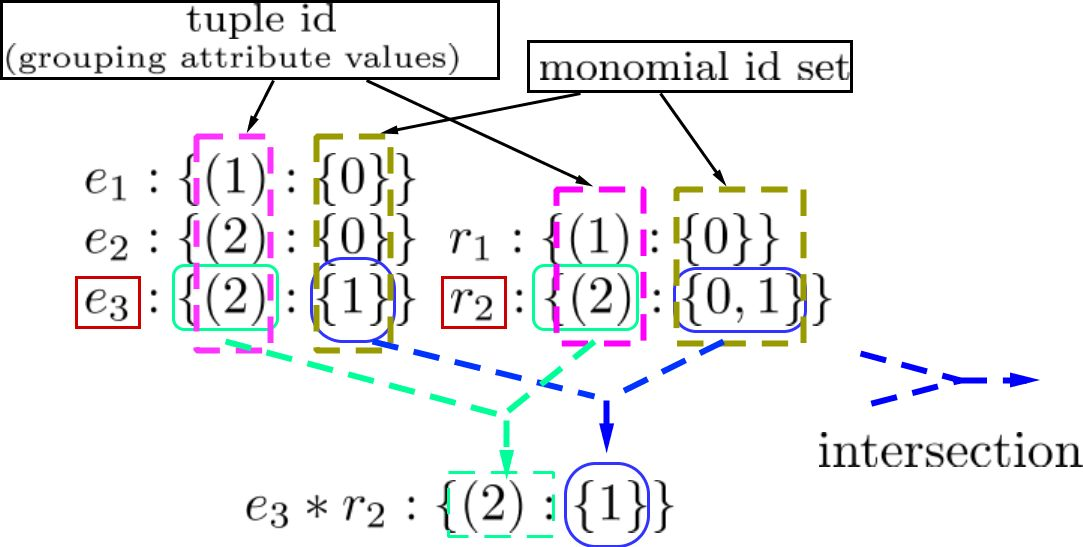
\includegraphics[width=0.4\textwidth,height=0.2\textwidth]{Figures/intersection.jpg}
    \caption{Query provenance index for $Q$ and how to compute coordinate for $e_3*r_2$ from $V_4(D)$}
    \small \label{fig:query prov index}
\end{figure}

In the {\em Reasoning} step, since $V_3$ is a {conjunctive view}, the validity of $M_3$ for a query tuple $t_q$ only depends on the {\em existence} of $t_q$ in $V_3(D)$ under mapping $M_3$ (Section \ref{sec: conjunctive_example}). So we can simply retrieve the base relation tuple for each provenance token appearing in the query to evaluate the view {predicates}. For example, the validity of $M_3$ can be checked simply by examining the predicates of $V_3$. Since the first predicate in $V_3$, $T = T'$, is also in $Q$, every tuple in the query instance must satisfy it. However, the second predicate, $E \leq 2$, can affect the {existence} of query tuples in $V_3$. Table \ref{Instance of Exon} shows that only the tuples with how-provenance tokens $e_1$ and $e_2$ satisfy $E \leq 2$. Thus $M_3$ is only valid for $t_{{q}1}$, whose how-provenance polynomial only includes $e_1$. %without any other how-provenance tokens from Exon.
{Note that the implementation used here is different from \rba\ since evaluating view predicates is achieved by {referencing the base relation tuples with the query provenance} rather than computing extra predicates in the query evaluation.}  
%This difference in performance will be discussed in Section \ref{sec:experiments}.

\begin{table}
\centering
\small
\caption{$V_4(D)$ with how-provenance polynomials}\label{Instance of V4}
\vspace*{-0.2cm}
% \begin{tabular}[t]{c|c|c|c||b|} \hhline{~----}
% &T1&N1&COUNT(E)&prov\\ \hhline{~----}
% $t_{v_41}$&4&HP-218&1&$e_4*r_3$\\ \hhline{~----}
% $t_{v_42}$&5&GK-207&2&$e_6*r_4 + e_7*r_4$\\ \hhline{~----}
% \end{tabular}
\begin{tabular}[t]{c|c|c||b|} \hhline{~---}
&G1&COUNT(T1)&prov\\ \hhline{~---}
$t_{v_41}$&1&1&$e_1*r_1$\\ \hhline{~---}
$t_{v_42}$&3&1&\makecell{$e_3*r_2 + e_4*r_2$}\\ \hhline{~---}
\end{tabular}
\medskip
\caption{$V_5(D)$ with how-provenance polynomials}\label{Instance of V5}
\vspace*{-0.2cm}
% \begin{tabular}[t]{c|c|c|c||b|} \hhline{~----}
% &T1&N1&MAX(L)&prov\\ \hhline{~----}
% $t_{v_51}$&1&MB-203&1&$e_1*r_1$\\ \hhline{~----}
% $t_{v_52}$&2&PC-203&3&$e_2*r_2 + e_3*r_2$\\ \hhline{~----}
% $t_{v_53}$&4&HP-218&2&$e_4*r_3$\\ \hhline{~----}
% $t_{v_54}$&5&GK-207&3&$e_5*r_4 + e_6*r_4 + e_7*r_4$\\ \hhline{~----}
% \end{tabular}
\begin{tabular}[t]{c|c|c|c||b|} \hhline{~----}
&G1&MAX(L)&COUNT(E)&prov\\ \hhline{~----}
$t_{v_51}$&1&1&1&$e_1*r_1$\\ \hhline{~----}
$t_{v_52}$&2&3&2&\makecell{$e_2*r_2 + e_3*r_2$\\$ + e_4*r_2$}\\ \hhline{~----}
% $t_{v_53}$&3&3&2&\makecell{$e_4*r_3 + e_5*r_4$}\\ \hhline{~----}
\end{tabular}
\medskip
\caption{$V_6(D)$ with how-provenance polynomials}\label{Instance of V6}
\vspace*{-0.2cm}
\begin{tabular}[t]{c|c|c||b|} \hhline{~---}
&G&COUNT(T)&prov\\ \hhline{~---}
$t_{v_61}$&1&1&$r_1$\\ \hhline{~---}
$t_{v_62}$&2&1&$r_2$\\ \hhline{~---}
% $t_{v_63}$&3&2&$r_3 + r_4$\\ \hhline{~---}
\end{tabular}
\medskip
\caption{$Q(D)$ with valid view mappings and covering sets (aggregate terms omitted)}\label{Instance of Q1 with view mappings}
\vspace*{-0.2cm}
\hspace*{-0.2cm}
\begin{tabular}[t]{c|c||c|c|} \hhline{~---}
&G&valid view mappings&covering sets\\ \hhline{~---}
$t_{q1}$&1&$M_3, M_4, M_5, M_6$&\makecell{$\{\{M_3\}, \{M_4, M_5\}$\\$, \{M_5, M_6\}\}$}\\ \hhline{~---}
$t_{q2}$&2&$M_6$&$\{\{M_6\}\}$\\ \hhline{~---}
% $t_{q3}$&3&$M_6$&$\{\{M_6\}\}$\\ \hhline{~---}
\end{tabular}
\end{table}

% \begin{figure}
% % \captionsetup[subfigure]{width=1\textwidth}
%      \centering
%     \begin{subfigure}{0.50\textwidth}
%     % \hspace*{-0.8cm}
%         \raisebox{-\height}{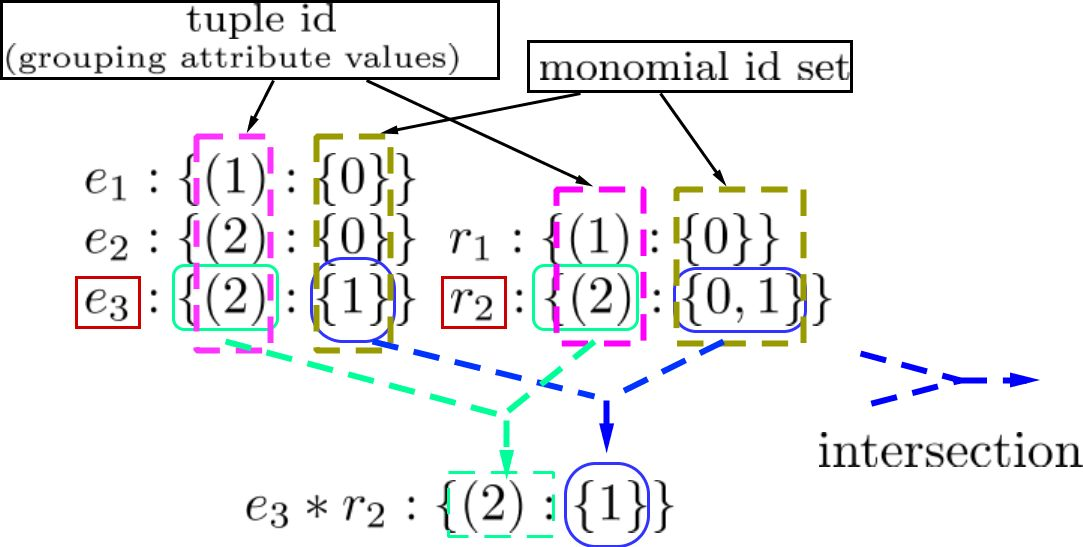
\includegraphics[height = 0.5\textwidth, width=1\textwidth]{Figures/intersection.jpg}}
%         \caption{query provenance index for $Q$ and computing coordinate information for $e_6*r_4$}     \label{fig:stress_test_instance_size}
%     \end{subfigure}
% \end{figure}
% \begin{table}[htp]
% \centering
% \small

% \end{table}

% \begin{table}[htp]
% \centering
% \small
% \caption{The instance of relation $Q_1$ along with how-provenance polynomials}\label{Instance of Q1}
% \begin{tabular}[t]{c|c|c|c|c|c|c|c|} \hhline{~-------}
% &T1&&N1&&COUNT(E)&MAX(L)&\\ \hhline{~-------}
% $t_{q_11}$&1&$\{t_1\}$&MB-203&$\{t_2\}$&1&1&$E_1*T_1$\\ \hhline{~-------}
% $t_{q_12}$&2&$\{t_5\}$&PC-203&$\{t_6\}$&2&3&$E_2*T_2 + E_3*T_2$\\ \hhline{~-------}
% $t_{q_13}$&4&$\{t_9\}$&HP-218&$\{t_6\}$&1&2&$E_4*T_3$\\ \hhline{~-------}
% $t_{q_14}$&5&$\{t_{13}\}$&GK-207&$\{t_6\}$&2&3&$E_5*T_4 + E_6*T_4$\\ \hhline{~-------}
% \end{tabular}
% \end{table}

% \begin{table}[htp]
% \centering
% \small

% \end{table}

% \begin{table}[htp]
% \centering
% \small
% \caption{The instance of relation $V5$}\label{Instance of V5}
% \begin{tabular}[t]{c|c|c|c|c|} \hhline{~----}
% &T1&N1&MAX(L)&\\ \hhline{~----}
% $t_{v_51}$&1&MB-203&1&$\{\{E_1,T_1\}\}$\\ \hhline{~----}
% $t_{v_52}$&2&PC-203&3&$\{\{E_2,T_2\}, \{E_3,T_2\}$\\ \hhline{~----}
% $t_{v_53}$&4&HP-218&2&$\{\{E_4,T_3\}\}$\\ \hhline{~----}
% $t_{v_54}$&5&GK-207&3&$\{\{E_5,T_4\}, \{E_6,T_4\}, \{E_7,T_4\}\}$\\ \hhline{~----}
% \end{tabular}
% \end{table}

% \begin{table}[htp]
% \centering
% \small

% \end{table}

In contrast, since $V_4$, $V_5$ and $V_6$ are aggregate views, we need to compare their how-provenance expressions with the how-provenance of the query to check the {tuple-level conditions}. That can be naively implemented by scanning the entire query provenance for {\em every view mapping} to build satisfiable provenance mappings (Def. \ref{Def: validity condition agg}), which is expensive when $N_{pv}$, $N_{pq}$ and the number of view mappings $m$ are large.  To reduce this cost, we index the query provenance.

\textbf{Query provenance index optimization.} 
% \scream{very long sentence. Please simplify}. 
\eat{Hashmap (mapping the grouping attribute values to the how-provenance monomial set for each query tuple) seems to be helpful to speed up the searching, which, however, still needs to scan the entire query provenance for every view mapping for initialization since the portion of how-provenance monomials in the query {\em involved} in the view mappings may be varied across different view mappings. For example, the view mapping $M_6$ only covers the subgoal $Transcript$ in the query body and thus only the provenance token $r_x (x=1,2,...)$ should be {\em involved} in $M_6$. However, both the token $r_x$ and $e_y$ are {\em involved} in $M_4$ and $M_5$. Such difference can lead to totally different HashMaps and thus inevitable repetitive scans over the entire query provenance for every view mapping in the worst case.}
In order to avoid multiple scans over query provenance, we build an index $I$ for each token in the query provenance to indicate which query tuples (represented by grouping variable values) and which provenance monomials the token is in. The provenance index for $Q$ is shown in Figure \ref{fig:query prov index}. For example, referencing Table \ref{Instance of Q1}, note that token $r_2$ is in the $0^{th}$ and $1^{st}$ monomial in the query tuple $t_{q2}$, which has value $2$ for the grouping variable $G$. So the index for $r_2$ is $r_2:\{(2):\{0,1\}\}$, where $(2)$ represents the tuple id while $\{0,1\}$ is the monomial id set. For a how-provenance monomial in the view, e.g. $e_3*r_2$ in $t_{v_42}$ (with grouping variable value 2), to determine whether it can be mapped to some query provenance monomial, we can retrieve the index for $e_3$ and $r_2$ with grouping variable value $2$ respectively, i.e. $\{1\}$ and $\{0,1\}$, and take the intersection, i.e. $\{1\}$. This indicates that $e_3$ and $r_2$ coexist in the $1^{st}$ monomial of the query tuple with grouping variable value 2 (i.e. $t_{q2}$). 
This derivation process is highlighted in Figure \ref{fig:query prov index}.

We can further optimize the intersection operation by representing the monomial ids with bit arrays, where the $i^{th}$ bit is 0/1 iff a token is/isn't in the $i^{th}$ monomial, and applying bit AND operations. This strategy only requires one full scan over the query provenance to build an index for all view mappings. Details on how to use the index to determine whether provenance mappings from view tuples to query tuple satisfy Def. \ref{Def: validity condition agg} are presented in Algorithm \ref{reasoning_valid_view_mappings}.

\begin{algorithm}[h!] 
\footnotesize
 \SetKwInOut{Input}{Input}
 \SetKwInOut{Output}{Output}
 \Input{a view $V$, a query $Q$, a view mapping $M$ from $V$ to $Q$, query tuple $t_q \in Q(D)$, query provenance index $I$, a set of view tuples $T_v \subseteq V(D)$}

 \Output{Whether provenance mappings from $T_v$ to $t_q$ satisfy Def. \ref{Def: validity condition agg}}
 
\For{$t_v \in T_v$}
{
    Retrieve the provenance monomial set $\Bar{P}$ of $t_v$
    Retrieve the grouping variable values ($Gv$) of $Q$ under mapping $M$

    \For{each provenance monomial $P \in \Bar{P}$}
    {
        \For{each provenance token $p \in P$}
        {
            \If{$p$ is not in $I$ OR $Gv$ is not in the entry of $I$ for $p$}
            {
                \Return false
            }
            
        }
        
        Perform intersection over the index for $p$ with grouping variable values $Gv$
        
        \If{the intersection result is empty}
        {
            \Return false
        }
    }
    
}

\Return true

% {\em Preprocessing step}: Return a set of all possible view mappings $\mathcal{M}$ and the provenance of $Q$

% {\em Reasoning valid view mapping step}: Retrieve provenance of every view. For each query tuple $t$, determine valid view mappings by comparing the provenance of $Q$ and the provenance of $V$

% {\em Covering sets calculation step}: Calculate covering sets by combining valid view mappings for each query tuple.
%  \Return $\mathcal{M}$
 \caption{Checking provenance mappings}
 \label{reasoning_valid_view_mappings}
 \end{algorithm}





\begin{algorithm}[h!] 
\footnotesize
 \SetKwInOut{Input}{Input}
 \SetKwInOut{Output}{Output}
 \Input{a set of valid view mappings $\mathcal{M}$ for query tuple $t \in Q(D)$, query $Q$}

 \Output{a set of covering sets $C$}
 
 For each aggregate term of $Q$, derive a set of view mappings covering it, which forms an array of view mapping sets $S$. 
 
%  Constructing an array of view mapping set $S$ where each view mapping set covers the same aggregate attribute
 
 Determine the order to compute the cross product of every element in $S$
 
 Initialize $C$ as the first view mapping set $s_0$ from $S$.
 
 \For{each set $s\in S - \{s_0\}$}
 {
    
    Initialize cross product result $C' = \{\}$:
    
    \For{each view mapping set $\Bar{M}' \in C$}
    {
        \For{each view mapping $M \in s$}
        {
            get three bit arrays of $\Bar{M}'$ ($M$): $b_1$ ($b_1'$), $b_2$($b_2'$) and $b_3$ ($b_3'$)
            
            construct new view mapping set $\Bar{M}''$ based on the bit OR operation result $b_i \lor b_i' (i=1,2,3)$ and put it into $C'$
        }
    }
    
    
    
    Remove duplicates from $C'$
    
    $C = C'$
    
 }
 
 \caption{Compute covering sets}
 \label{compute_covering_sets}
 \end{algorithm}




\textbf{Materialization and parallelism optimization.} To further improve performance, the provenance of the aggregate views along with the view content can be materialized before the query arrives. The strategy with  materialized view provenance is called {\em eager}, whereas that without is called {\em lazy}. The {\em eager} and {\em lazy} strategies are compared in Section \ref{sec:experiments}. We observe that reasoning about the validity of view mappings is highly parallelizable since the reasoning between different view mappings is independent.
However, since fully parallel computation in a single machine can incur large memory consumption, ProvCite only processes five view mappings at a time. Exploring how to fully develop our system in a distributed environment is left for future work.

% and which can be dealt with by two alternative strategies. One is to pre-compute their how-provenance ({\em eager strategy}) while the other one is to retrieve their how-provenance on the fly ({\em lazy strategy}). Their trade-offs will be discussed in Section~\ref{sec:experiments}.

Using the instances and provenance expressions of $V_4-V_6$ presented in Tables \ref{Instance of V4}-\ref{Instance of V6}, the valid view mappings for every query tuple are presented in Table \ref{Instance of Q1 with view mappings}. Note that for tuple $t_{q2}$, although all of its how-provenance monomials exist in the view tuple $t_{v_52}$, it does not include $e_4*r_2$ which is used to construct $t_{v_52}$, violating the {tuple-level condition}.  Intuitively, since the value of the aggregate term may come from this component of the monomial ($e_4*r_2$), $t_{v_52}$ should not provide citation information for $t_{q2}$.

Finally, valid view mappings are shown in Table \ref{Instance of Q1 with view mappings} along with the query instance, which are then used to compute covering sets for each query tuple in the {\em Covering sets step}. 
\eat{Note that for tuple $t_{{q}3}$, there are two covering sets, $\{M_3\}$ and $\{M_4, M_5\}$;  
% both of these sets cover the aggregate terms in $Q_1$ and are combined using $*$ and $+^R$. % as Table \ref{Instance of Q1 with view mappings} shows. covers both the aggregate terms in $Q1$. 
other combinations of view mappings either {redundantly} or {non-maximally} cover the query's aggregate terms, and therefore are not valid.}


As we observed in \cite{wu2018data}, it is time-consuming to compute {\em all} covering sets. We therefore use two new strategies to achieve speed-up: 1) representing coverings sets using bit arrays; and 2) applying clustering algorithms to avoid an explosion of intermediate results.  These lead to an order of magnitude performance gain (see Section \ref{sec:experiments}).

% \subsubsection{Introducing bit arrays}
\textbf{Bit array optimization.} The computation of covering sets involves merging valid view mappings and removing duplicates, which can be optimized using bit operations. For example, for $Q$, the aggregate term $COUNT(T)$, $MAX(L)$ and $COUNT(E)$ are covered by $\{M_3, M_4, M_6\}$ (denoted by $S_1$), $\{M_3, M_5\}$ (denoted by $S_2$) and $\{M_3, M_5\}$ (denoted by $S_3$) respectively (see Table \ref{Table: view mapping coverage}). We can encode the $0^{th}-3^{rd}$ view mappings $M_3-M_6$ as $\{0,1,2,3\}$, the $0^{th}-2^{nd}$ aggregate terms ($COUNT(T)$, $MAX(L)$ and $COUNT(E)$) as $\{0, 1, 2\}$, and the $0^{th}-1^{st}$ relational subgoals ($Exon$ and $Transcript$) as $\{0, 1\}$.  In this manner, arbitrary view mapping combinations (and thus covering sets) can be represented using three bit arrays in which the $i^{th}$ bit is 1 (0) iff the $i^{th}$ view mapping is included (missing), or the $i^{th}$ aggregated term or relational subgoal is covered (not covered). 
For example, $M_4$ is the $1^{st}$ view mapping, represented by $0100$ (the leftmost bit is the $0^{th}$ bit). $M_4$ covers the $0^{th}$ aggregate term $(COUNT(T))$ and the $0^{th}$ and $1^{st}$ relational subgoals, which are represented by bit arrays $100$ and $11$ respectively. The bit array representations for other view mappings are listed in Table \ref{Table: view mapping}. To compute covering sets, the view mapping combinations from the cross product of $\{S_1, S_2, S_3\}$ (denoted by $S_1 \times S_2 \times S_3$) are considered, which are constructed by applying bit OR operations over the bit arrays from those view mappings. For example, referencing Table \ref{Table: view mapping}, the covering set $\{M_4, M_5\}$ can be constructed by unioning bit arrays $0100$ and $0010$, and the aggregate terms (relational subgoals resp.) jointly covered by them are computed by unioning $100$ and $011$ ($11$ and $11$ resp.). The pseudocode for computing covering sets using bit array representations is presented in Algorithm \ref{compute_covering_sets}.

% To compute covering sets, the cross product of $S_1$ and $S_2$ are computed first, which leads to some view mapping combinations (called {\em sub-covering sets thereafter}) that can cover both the aggregate terms. For instance, $\{M_3, M_5\}$ is one such sub-covering set. The construction of sub-covering sets (and covering sets ultimately) involves merging the view mappings and the aggregate terms and relational subgoals covered by them, which facilitate the following redundancy removal step. For example, $\{M_3,M_6\}$ (picked from $S_1$ and $S_2$ respectively) can jointly cover both the aggregate terms and relational subgoals of $Q$, which, however, is redundant with respect to $\{M_6\}$ (picked from $S_1$ and $S_2$ and one copy is retained) since $\{M_6\}$ is a {\em subset} of $\{M_3,M_6\}$ but still covers the same aggregate terms and relational subgoals as $\{M_3,M_6\}$. So it is safe to remove $\{M_3, M_6\}$ at this point. Then the resulting sub-covering sets are combined with the view mapping set in $S_3$ to compute the final covering sets.

% Note that two key operations are essential in this step, i.e. 1) merging view mappings and the terms covered by them; 2) removing redundancy by subset checking, which can be optimized by applying bit operations.  Three bit arrays are introduced for view mapping combinations, aggregate terms and relational subgoals, in which $i_th$ bit is 0 or 1 if $i_th$ view mapping/aggregate term/relational subgoal is included or missing in the sub-covering set. For example, for sub-covering set $\{M_3, M_6\}$, we use bit array 1001 to represent the view mapping in it (the leftmost 1 is in the 0th bit, which indicates the existence of $M_3$). Similarly, since they cover both the aggregate terms and relational subgoals, the other two bit arrays will be both 11. So when merging sub-covering set (or view mappings) with other sub-covering set (or view mappings), we can apply bit OR operations over the three bit arrays. Similarly, for subset checking operation, bit AND operation is applicable.



% \subsubsection{Applying clustering algorithms}
\textbf{Clustering algorithm optimization.} Since cross product ($\times$) is commutative and associative, different orderings of operands result in the same output but may incur different overhead. For example, with $S_1\times S_2 \times S_3$, if $S_2 \times S_3$ is computed first, the result is $\{M_3, M_5\}$, $\{M_5, M_5\}$, $\{M_3, M_3\}$, $\{M_5, M_3\}$. After removing obvious redundancy, the result is  $\{M_3, M_5\}$, $\{M_5\}$, $\{M_3\}$. Note that $\{M_3, M_5\}$ is a duplicate compared to $\{M_3\}$ since 1) $\{M_3, M_5\}$ and $\{M_3\}$ cover the same set of aggregate terms and relational subgoals (checked by comparing the corresponding bit arrays); and 2) $\{M_3\}$ is a subset of $\{M_3, M_5\}$. It is therefore safe to remove $\{M_3, M_5\}$ since in the final result, any view mapping combinations which include $\{M_3, M_5\}$ will be a duplicate compared to one that includes $\{M_3\}$ and thus won't be a covering set. So the intermediate result of $S_2 \times S_3$ is $\{\{M_3\}, \{M_5\}\}$, which is smaller than the result of the other pairs. This is due to the high similarity between $S_2$ and $S_3$ (actually $S_2 = S_3$). To find good orderings for computing the cross product such that the intermediate result is minimized, clustering algorithms are applied so that view mapping sets which are similar to each other can be clustered and merged first (e.g. $S_2$ and $S_3$). In ProCite, the affinity propagation clustering algorithm \cite{dueck2007non} is used since it does not require a pre-specified number of clusters.
\end{example}